
%(BEGIN_QUESTION)
% Copyright 2011, Tony R. Kuphaldt, released under the Creative Commons Attribution License (v 1.0)
% This means you may do almost anything with this work of mine, so long as you give me proper credit

Suppose you did a competent job of installing a positioner on a control valve, including careful alignment of the feedback linkage where the positioner connects to the valve stem.  However, after you completed your job, the valve got passed on to someone who knew nothing about positioners.  That person mis-aligned the linkage connecting the positioner to the valve stem, moving the travel pin to a new position (further up than it should be).  Compare the illustrations below for a ``before-and-after'' comparison:

$$\includegraphics[width=15.5cm]{i01448x01.eps}$$

\noindent
Examine these two illustrations, and then answer the following questions:

\begin{itemize}
\item{} Supposing the former calibration of this positioner was 4 mA (fully shut) to 20 mA (fully open), choose the most likely calibration range the valve now exhibits:
\itemitem{} Shut at 2 mA, fully open at 18 mA
\itemitem{} Shut at 2 mA, fully open at 22 mA
\itemitem{} Shut at 6 mA, fully open at 22 mA
\itemitem{} Shut at 6 mA, fully open at 18 mA
\vskip 10pt
\item{} Explain why this calibration error caused by linkage mis-alignment cannot be corrected simply by adjusting the positioner's zero and/or span controls.  In other words, what problem(s) will remain even after re-zeroing and re-spanning the positioner (without re-aligning the linkage)?
\end{itemize}


\underbar{file i01448}
%(END_QUESTION)





%(BEGIN_ANSWER)

Half-credit for each correct answer:

\vskip 10pt

\itemitem{} {\bf Shut at 6 mA, fully open at 22 mA}

\vskip 10pt

Multiple problems will result from this mis-alignment of the feedback arm.  Grant credit for {\it any} of the following answers, or any other valid conclusions reached by the student:

\begin{itemize}
\item{} Even after re-zeroing and re-spanning the positioner, the valve will not respond {\it linearly} anymore, since the initial angle is all wrong.
\item{} The positioner arm's rated travel will likely be exceeded as the valve goes to its full-open position.  This may damage the positioner, as well as lead to unstable valve behavior toward the full-open position.
\end{itemize}


%(END_ANSWER)





%(BEGIN_NOTES)

{\bf This question is intended for exams only and not worksheets!}.

%(END_NOTES)


